% Chapter 1

\chapter{MicroRNAs and their importance in living beings} % Main chapter title

\label{Chapter1} % For referencing the chapter elsewhere, use \ref{Chapter1} 

%----------------------------------------------------------------------------------------

% Define some commands to keep the formatting separated from the content 
\newcommand{\keyword}[1]{\textbf{#1}}
\newcommand{\tabhead}[1]{\textbf{#1}}
\newcommand{\code}[1]{\texttt{#1}}
\newcommand{\file}[1]{\texttt{\bfseries#1}}
\newcommand{\option}[1]{\texttt{\itshape#1}}

%----------------------------------------------------------------------------------------

\section{What are microRNAs?}
MicroRNAs (abbreviated miRNAs) are a family of $\approx 22$-nucleotide small non-coding RNAs that regulates gene expression at the post-transcriptional level \cite{mirna_intro}. This means that they act by binding to partially complementary sites on target genes, which had been previously transcribed from the DNA of the cell, to induce cleavage or repression of productive translation, preventing this way the target gene to be able to exit the cell and start the translational process that produces peptides and proteins.

\begin{figure}[hbt!]
	\centering
	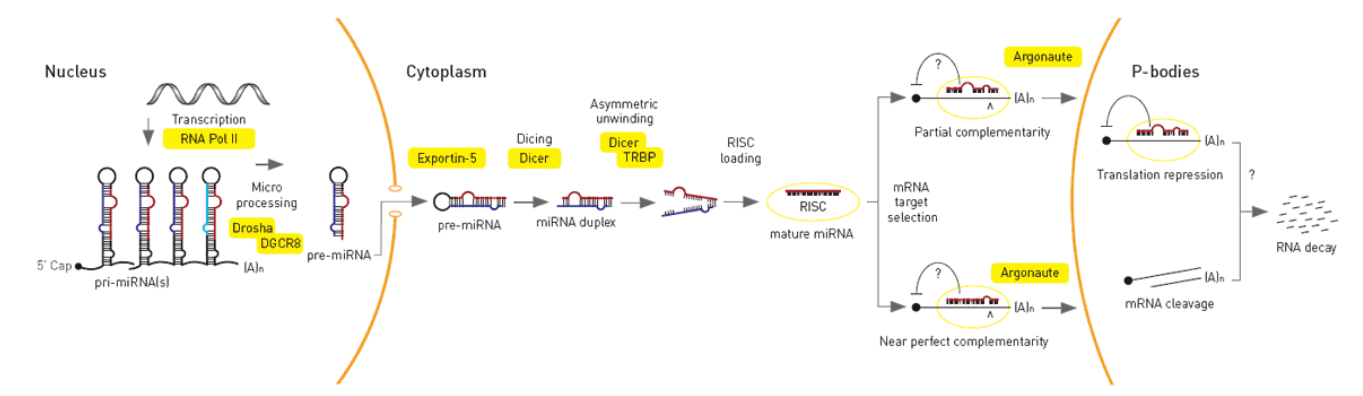
\includegraphics[width=1.0\textwidth]{Figures/mirna_genesis}
	\caption{MiRNAs genesis and functionalities}
	\label{fig:mirna_genesis}
\end{figure}

\subsection{Transcription and processing of miRNAs}
As shown in figure \ref{fig:mirna_genesis} miRNAs genes are transcribed by the RNA polymerase II as as large primary transcripts (pri-miRNA) that are processed by a protein complex containing the enzyme Drosha, to form an approximately 70 nucleotide precursor miRNA (pre-miRNA). This precursor is subsequently transported to the cytoplasm where it is processed by a second enzyme, called DICER, to form a mature miRNA of approximately 22 nucleotides. The mature miRNA is then incorporated into a ribonuclear particle to form the RNA-induced silencing complex, RISC, which mediates gene silencing.

It's important to note that, generally, only one of the two strands of the stem loop is incorporated into the silencing process, and it's selected on the basis of its thermodynamic instability and weaker base-pairing on the 5' end relative to the other strand. The latter, called the passenger strand due to its lower levels in the steady state, is usually denoted with an asterisk (*) and is normally degraded. However, in some cases, both strands of the duplex are viable and become functional miRNAs that target different mRNA populations. (see figure \ref{fig:mirna_stems})

\begin{figure}[hbt!]
	\centering
	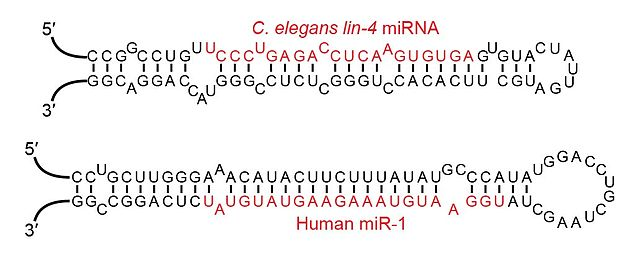
\includegraphics[width=1.0\textwidth]{Figures/mirna_stems}
	\caption{Examples of miRNA stem-loops. In red is shown the mature miRNA}
	\label{fig:mirna_stems}
\end{figure}

\subsection{RNA-induced silencing complex (RISC)}
As mentioned before the mature miRNA is part of an active RNA-induced silencing complex (RISC). This process represents their main functionality in both animals and plants. 
The RISC it is a key process in gene silencing and can act in two different ways as depicted in the right-hand side of picture \ref{fig:mirna_genesis}: via mRNA degradation or by preventing mRNA translation. It has been demonstrated that given complete complementarity between the miRNA and target mRNA sequence, Ago2 can cleave the mRNA and lead to direct mRNA degradation. In the presence of only partial complementarity instead, silencing is achieved by preventing translation \cite{cleavage}.
 
%----------------------------------------------------------------------------------------

\section{Why are they important?}
MiRNAs are particularly abundant in many mammalian cell types and appear to target about 60\% of the genes of humans and other mammals \cite{conserved_pairing}.

Many miRNAs are evolutionarily conserved, which implies that they have important biological functions \cite{conserved_pairing}. For example, 90 families of miRNAs have been conserved since at least the common ancestor of mammals and fish, and most of these conserved miRNAs have important functions.

The discovery of the first miRNA over 20 years ago has ushered in a new era in molecular biology. There are now over 2000 miRNAs that have been discovered in humans and it is believed that they collectively regulate two third of the genes in the genome.

The repressive action of miRNAs has a huge impact on many biological processes such as cell cycle control and several developmental and physiological processes including stem cell differentiation, cardiac and skeletal muscle development, neurogenesis, insulin secretion, cholesterol metabolism, aging, immune responses and viral replication. \cite{mirna_annotation}

In addition to their important roles in healthy individuals, microRNAs have also been implicated in a number of diseases including a broad range of cancers, heart and neurological diseases.  In fact it has been discovered that their expression patterns  are highly specific in respect to external stimuli, developmental stage or tissue and this can be used to diagnose diseases in which the expression levels of miRNAs are known to change considerably \cite{computational_methods}. Consequently, miRNAs are intensely studied as candidates for clinical diagnosis and predictors of drug response \cite{mirna_diseases}.

\section{Why miRNAs target prediction is a difficult task?}




\section{acaso}

\subsection{Folders}

This template comes as a single zip file that expands out to several files and folders. The folder names are mostly self-explanatory:

\keyword{Appendices} -- this is the folder where you put the appendices. Each appendix should go into its own separate \file{.tex} file. An example and template are included in the directory.

\keyword{Chapters} -- this is the folder where you put the thesis chapters. A thesis usually has about six chapters, though there is no hard rule on this. Each chapter should go in its own separate \file{.tex} file and they can be split as:
\begin{itemize}
\item Chapter 1: Introduction to the thesis topic
\item Chapter 2: Background information and theory
\item Chapter 3: (Laboratory) experimental setup
\item Chapter 4: Details of experiment 1
\item Chapter 5: Details of experiment 2
\item Chapter 6: Discussion of the experimental results
\item Chapter 7: Conclusion and future directions
\end{itemize}

%---------------------------------------------------------------------------------------

\subsection{Tables}

Tables are an important way of displaying your results, below is an example table which was generated with this code:

{\small
\begin{verbatim}
\begin{table}
\caption{The effects of treatments X and Y on the four groups studied.}
\label{tab:treatments}
\centering
\begin{tabular}{l l l}
\toprule
\tabhead{Groups} & \tabhead{Treatment X} & \tabhead{Treatment Y} \\
\midrule
1 & 0.2 & 0.8\\
2 & 0.17 & 0.7\\
3 & 0.24 & 0.75\\
4 & 0.68 & 0.3\\
\bottomrule\\
\end{tabular}
\end{table}
\end{verbatim}
}

\begin{table}
\caption{The effects of treatments X and Y on the four groups studied.}
\label{tab:treatments}
\centering
\begin{tabular}{l l l}
\toprule
\tabhead{Groups} & \tabhead{Treatment X} & \tabhead{Treatment Y} \\
\midrule
1 & 0.2 & 0.8\\
2 & 0.17 & 0.7\\
3 & 0.24 & 0.75\\
4 & 0.68 & 0.3\\
\bottomrule\\
\end{tabular}
\end{table}

You can reference tables with \verb|\ref{<label>}| where the label is defined within the table environment. See \file{Chapter1.tex} for an example of the label and citation (e.g. Table~\ref{tab:treatments}).


There are many different \LaTeX{} symbols to remember, luckily you can find the most common symbols in \href{http://ctan.org/pkg/comprehensive}{The Comprehensive \LaTeX~Symbol List}.

You can write an equation, which is automatically given an equation number by \LaTeX{} like this:
\begin{verbatim}
\begin{equation}
E = mc^{2}
\label{eqn:Einstein}
\end{equation}
\end{verbatim}

This will produce Einstein's famous energy-matter equivalence equation:
\begin{equation}
E = mc^{2}
\label{eqn:Einstein}
\end{equation}

All equations you write (which are not in the middle of paragraph text) are automatically given equation numbers by \LaTeX{}. If you don't want a particular equation numbered, use the unnumbered form:
\begin{verbatim}
\[ a^{2}=4 \]
\end{verbatim}

%----------------------------------------------------------------------------------------

\section{In Closing}

You have reached the end of this mini-guide. You can now rename or overwrite this pdf file and begin writing your own \file{Chapter1.tex} and the rest of your thesis. The easy work of setting up the structure and framework has been taken care of for you. It's now your job to fill it out!

Good luck and have lots of fun!

\begin{flushright}
Guide written by ---\\
Sunil Patel: \href{http://www.sunilpatel.co.uk}{www.sunilpatel.co.uk}\\
Vel: \href{http://www.LaTeXTemplates.com}{LaTeXTemplates.com}
\end{flushright}
